%%%%%%%%%%%%%%%%%%%%%%%%%%%%%%%%%%%%%%%%%
% Stylish Article
% LaTeX Template
% Version 2.1 (1/10/15)
%
% This template has been downloaded from:
% http://www.LaTeXTemplates.com
%
% Original author:
% Mathias Legrand (legrand.mathias@gmail.com) 
% With extensive modifications by:
% Vel (vel@latextemplates.com)
%
% License:
% CC BY-NC-SA 3.0 (http://creativecommons.org/licenses/by-nc-sa/3.0/)
%
%%%%%%%%%%%%%%%%%%%%%%%%%%%%%%%%%%%%%%%%%

%----------------------------------------------------------------------------------------
%	PACKAGES AND OTHER DOCUMENT CONFIGURATIONS
%----------------------------------------------------------------------------------------

\documentclass[fleqn,10pt]{SelfArx} % Document font size and equations flushed left

\usepackage[T1]{fontenc}

% \usepackage{microtype}

\usepackage[english]{babel} % Specify a different language here - english by default

\usepackage{lipsum} % Required to insert dummy text. To be removed otherwise

%----------------------------------------------------------------------------------------
%	COLUMNS
%----------------------------------------------------------------------------------------

\setlength{\columnsep}{0.55cm} % Distance between the two columns of text
\setlength{\fboxrule}{0.75pt} % Width of the border around the abstract

%----------------------------------------------------------------------------------------
%	COLORS
%----------------------------------------------------------------------------------------

\definecolor{color1}{RGB}{0,0,90} % Color of the article title and sections
\definecolor{color2}{RGB}{0,20,20} % Color of the boxes behind the abstract and headings

%----------------------------------------------------------------------------------------
%	HYPERLINKS
%----------------------------------------------------------------------------------------

\usepackage{hyperref} % Required for hyperlinks
\hypersetup{hidelinks,colorlinks,breaklinks=true,urlcolor=color2,citecolor=color1,linkcolor=color1,bookmarksopen=false,pdftitle={Title},pdfauthor={Author}}

%----------------------------------------------------------------------------------------
%	ARTICLE INFORMATION
%----------------------------------------------------------------------------------------

\JournalInfo{Journal, Vol. XXI, No. 1, 1-5, 2013} % Journal information
\Archive{Additional note} % Additional notes (e.g. copyright, DOI, review/research article)

\PaperTitle{Visualization of Diffusion Limited Aggregation with OpenGL} % Article title

\Authors{Clayton Rayment\textsuperscript{1}} % Authors
% \affiliation{\textsuperscript{1}\textit{Department of Biology, University of Examples, London, United Kingdom}} % Author affiliation
% \affiliation{\textsuperscript{2}\textit{Department of Chemistry, University of Examples, London, United Kingdom}} % Author affiliation
% \affiliation{*\textbf{Corresponding author}: john@smith.com} % Corresponding author

\Keywords{DLA --- Visualization --- OpenGL} % Keywords - if you don't want any simply remove all the text between the curly brackets
\newcommand{\keywordname}{Keywords} % Defines the keywords heading name

%----------------------------------------------------------------------------------------
%	ABSTRACT
%----------------------------------------------------------------------------------------

\Abstract{An efficient single-threaded application for performing Diffusion Limited Aggregation simulations, along with a companion OpenGL visualizer using the GLUT GL Utility Toolkit. Particle-aggregator collisions are detected in $O(n \log n)$ time complexity, however this could be improved with the implementation of tree-based collision detection. }

%----------------------------------------------------------------------------------------

\begin{document}

\flushbottom % Makes all text pages the same height

\maketitle % Print the title and abstract box

\tableofcontents % Print the contents section

\thispagestyle{empty} % Removes page numbering from the first page

%----------------------------------------------------------------------------------------
%	ARTICLE CONTENTS
%----------------------------------------------------------------------------------------

\section*{Introduction} % The \section*{} command stops section numbering

\addcontentsline{toc}{section}{Introduction} % Adds this section to the table of contents

Diffusion Limited Aggregation is a simulation technique consisting of two basic particle types. Aggregator particles make up the first group of particles. An Aggregator particle does not move, and only interacts with the simulation when an Active Particle collides with it. The second group of particles, Active Particles, undergo a random walk at each timestep of the simulation. Should an Active Particle collide with an aggregator particle, the active particle will cease to be active, and become an aggregator particle in the location from where it collided. In this manner, an aggregate structure will grow as the simulation progresses. An example of such a structure can be seen in Figure 1.

\begin{figure}[ht]\centering % Using \begin{figure*} makes the figure take up the entire width of the page
    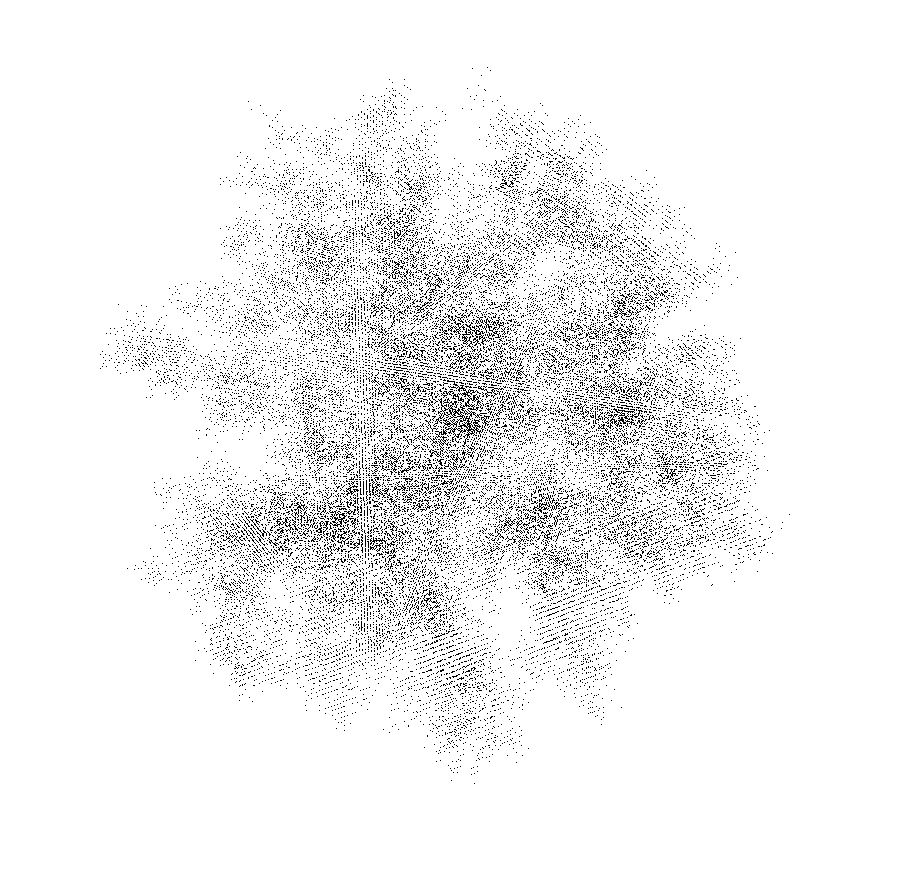
\includegraphics[width=\linewidth]{DLA45007-2-BW.png}
    \caption{Aggregate structure resulting from a DLA simulation using 50,000 particles. Aggregate structure shown contains 45,007 particles.}
    \label{fig:DLA45007}
    \end{figure}

%------------------------------------------------

\section{Implementation}
\subsection{Classes}
\subsubsection{Particle}
The \texttt{Particle} class is the most basic object of the simulation. The particle class defines only the location of the particle, the particle’s morton code, and functions to retreive/set these values. During the simulation, a particle will move randomly in one of eight possible directions by adding a random integer value [-1, 1] to each component of the particle’s position. Particles also contain a function which encodes the position into a 30-bit morton code, which is used to accelerate aggregation detection.
\subsubsection{Universe}
The \texttt{Universe} class is the overarching structure which contains all simulation operations. \texttt{Universe} contains an \texttt{std\allowbreak::vector} of all aggregated particles, and an \texttt{std\allowbreak::list} of all active particles. During each step of the simulation, the active particle list is iterated through, and each particle is moved, checking for collisions with the aggregate particles. For simplicity, collsions between active particles cannot occur, and the two particles will simply pass through eachother. 

\subsection{Fast Aggregate Lookup}
To speed up collision detection with the aggregate particles, each aggregate particle is assigned a Morton code based on the position of the particle. The \texttt{std\allowbreak::vector} container which holds all aggregator particles is then sorted using the aggregator particle's morton code.

During the collision check step, rather than search the entire aggregator particle vector looking for a particle that matches the position of the desired movement, Morton encoding allows the vector to sorted in a deterministic way, and searched using \texttt{std\allowbreak::binary\_serch}. This reduces the lookup time from $O(n)$ to $O(\log n)$.
\subsection{Visualizer}
\subsubsection{Overview}
Visualization is done using OpenGL. To increase performance, the visualizer is run in a separate thread using Pthreads. When the \texttt{Universe\allowbreak::renderUniverse()} method is called, the visualizer is started, and passed a pointer to the Universe class that called the visualizer.



\section{Operation}
\subsection{Aggregator Generation}
An aggregator file is a space-seperated value list containing only numbers in the following format:
\begin{center}
    \texttt{<X> <Y> <Z>}
\end{center}
Each line in the file represents a new aggregator particle in the system. Should the user not specify an imput aggregator file, there are several options available.
\subsection{Build Simulation}
Cmake files are included to automate the build process. From your build directory simply run
\begin{center}
    \texttt{cmake <dir>}
\end{center}
where \texttt{<dir>} is the path to the main \texttt{DLA/} directory which contains \texttt{CMakeLists.txt}. 
Then, from your build directory, simply run:
\begin{center}
    \texttt{make}
\end{center}
You will now find the executables in the \texttt{<dir>/bin/} directory.
\subsection{Run Simulation}
Once the project has been built, the simulation can be run from the command line using:
\begin{center}
    \texttt{<dir>/bin/simulation <Size> <Particles>}
\end{center}
\subsection{Output File}
\subsection{Visualizer}
Several options are available to the user from the visualizer, as displayed at the bottom of the visualization window:
\begin{description}
    \item[Esc] Close the simulation window and end the simulation.
    \item[F1] Toggle render mode between fast and fancy.\\ (Default: fast)
    \item[F2] Toggle bounding box to cover the simulation space.\\ (Default: off)
    \item[F3] Toggle rotation of camera around simulation.\\ (Default: off)
    \item[F4] Toggle visibility of active particles in simulation.\\ (Default: on)
\end{description}
An example of the visualizer window is shown in Figure 2.
\begin{figure}[ht]\centering % Using \begin{figure*} makes the figure take up the entire width of the page
    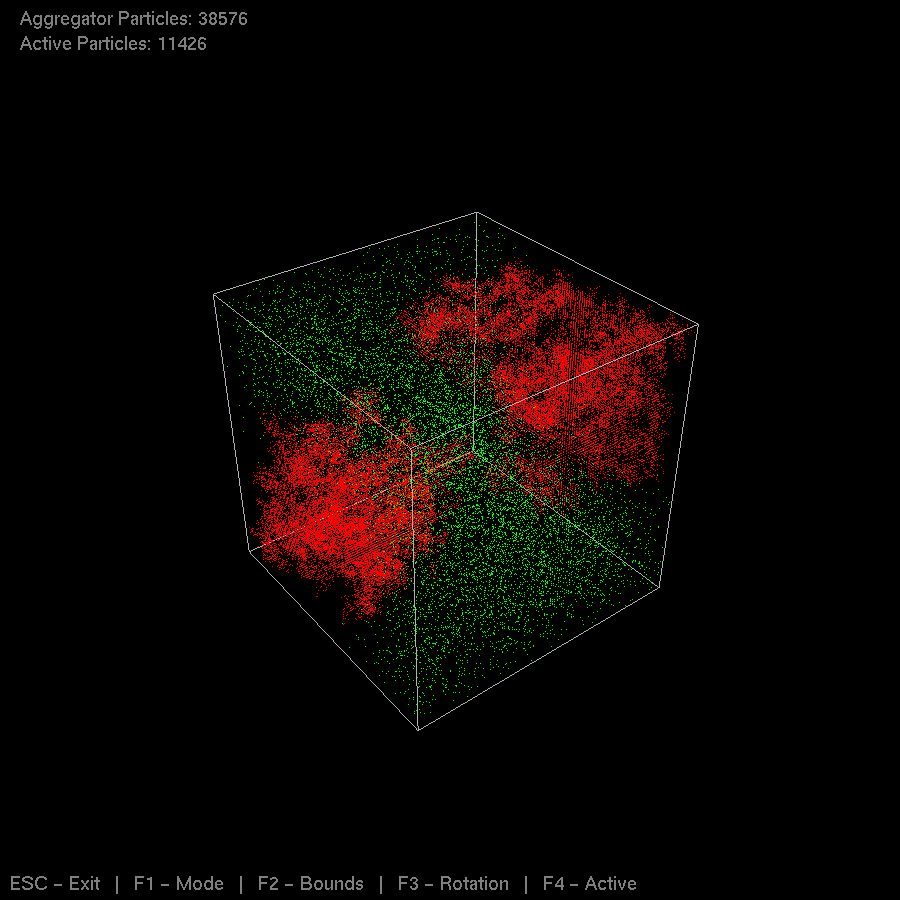
\includegraphics[width=\linewidth]{DLAVisualizer.png}
    \caption{DLA Visualizer application shown using fast graphics, bounding box, and active particles visible (green).}
    \label{fig:DLAAPP}
    \end{figure}
%------------------------------------------------



%------------------------------------------------
\phantomsection
\section*{Acknowledgments} % The \section*{} command stops section numbering
Morton Encoding code taken from \cite{Karras:2012}
%----------------------------------------------------------------------------------------
%	REFERENCE LIST
%----------------------------------------------------------------------------------------
\phantomsection
\bibliographystyle{unsrt}
\bibliography{references}

%----------------------------------------------------------------------------------------

\end{document}